\documentclass{article}
\usepackage[spanish]{babel}
\usepackage[utf8]{inputenc}
\usepackage[nonatbib]{../../template}

\usepackage[utf8]{inputenc} % allow utf-8 input
\usepackage[T1]{fontenc}    % use 8-bit T1 fonts
\usepackage{hyperref}       % hyperlinks
\usepackage{url}            % simple URL typesetting
\usepackage{booktabs}       % professional-quality tables
\usepackage{amsfonts}       % blackboard math symbols
\usepackage{nicefrac}       % compact symbols for 1/2, etc.
\usepackage{microtype}      % microtypography
\usepackage{xcolor}         % colors
\usepackage{graphicx}
\usepackage{float}
\usepackage[backend=biber,sorting=ynt,style=apa]{biblatex}

\addbibresource{bibliography.bib}

\graphicspath{ {../imagenes/} }

\title{Entrega 2: Metodología y EDA}

\author{%
  José Saint Germain\\
  \texttt{josesg998@gmail.com} \\
}

\begin{document}

\maketitle

\section{Introducción}
El objetivo de esta entrega es realizar una breve descripción de las metodologías que 
se utilizarán durante el trabajo final de especialización, así como realizar un 
análisis exploratorio de los datos (EDA), para comprender mejor la estructura de
los datos que se trabajarán.

\section{Metodología}
Como lo que buscamos realizar es experimentar con diferentes datos el mismo trabajo realizado
por el FMIm (\cite{Ceb24}), vamos a replicar las mismas técnicas de optimización de hiperparámetros, así como
los mismos algoritmos de entrenamiento y de intepretación de resultados.

Los algoritmos que se utilizarán serán Random Forest (\cite{Bre01}) y XGBoost
(\cite{Che16}). Para ajustar los hiperparámetros se utilizará la optimización
bayesiana junto al método de block-time-series cross-validation. Por último, la métrica a
optimizar y que se utilizará para comparar predicciones será el área bajo la curva (AUC).
Adicionalmente, se realizará un análisis exploratorio de datos de manera introductoria al
trabajo y se buscará utilizar valores Shapley para analizar los resultados de cada algoritmo.


\section{Análisis Exploratorio de Datos}

Como descripción general de la base de datos de VDEM, podemos mencionar que cuenta con 27734 filas y 4607 columnas. Como es una base de datos
de panel, se tiene información de 202 países durante 235 años. Para comprender la estructura de la información, es importante destacar que la base
original cuenta con información brindada por distintos expertos para cada país en cada año. Para poder procesar y obtener la base final, se agrega la información
de diferentes maneras. Es por este motivo que, además de la información identificactoria de cada país (la cual se repite en cada año), la mayoría de las variables
sustantivas cuentan con diferentes versiones, por cada tipo de variable de agregación generada. Por ejemplo, una variable puede contar con su versión princial, la cual
es un promedio reescalado del 1 al 5, sumado a una versión con la media simple (con sufijo _mean); una versión con el valor máximo y mínimo expresado por un experto
(_codehigh y codelow, respectivamente); y una versión con el desvío estándar (_sd), en caso de buscar conocer el grado de "acuerdo" entre los expertos respecto a
la situación del país.


\subsection{Ánalisis de nulos}
\begin{figure}[H]
  \centering  
  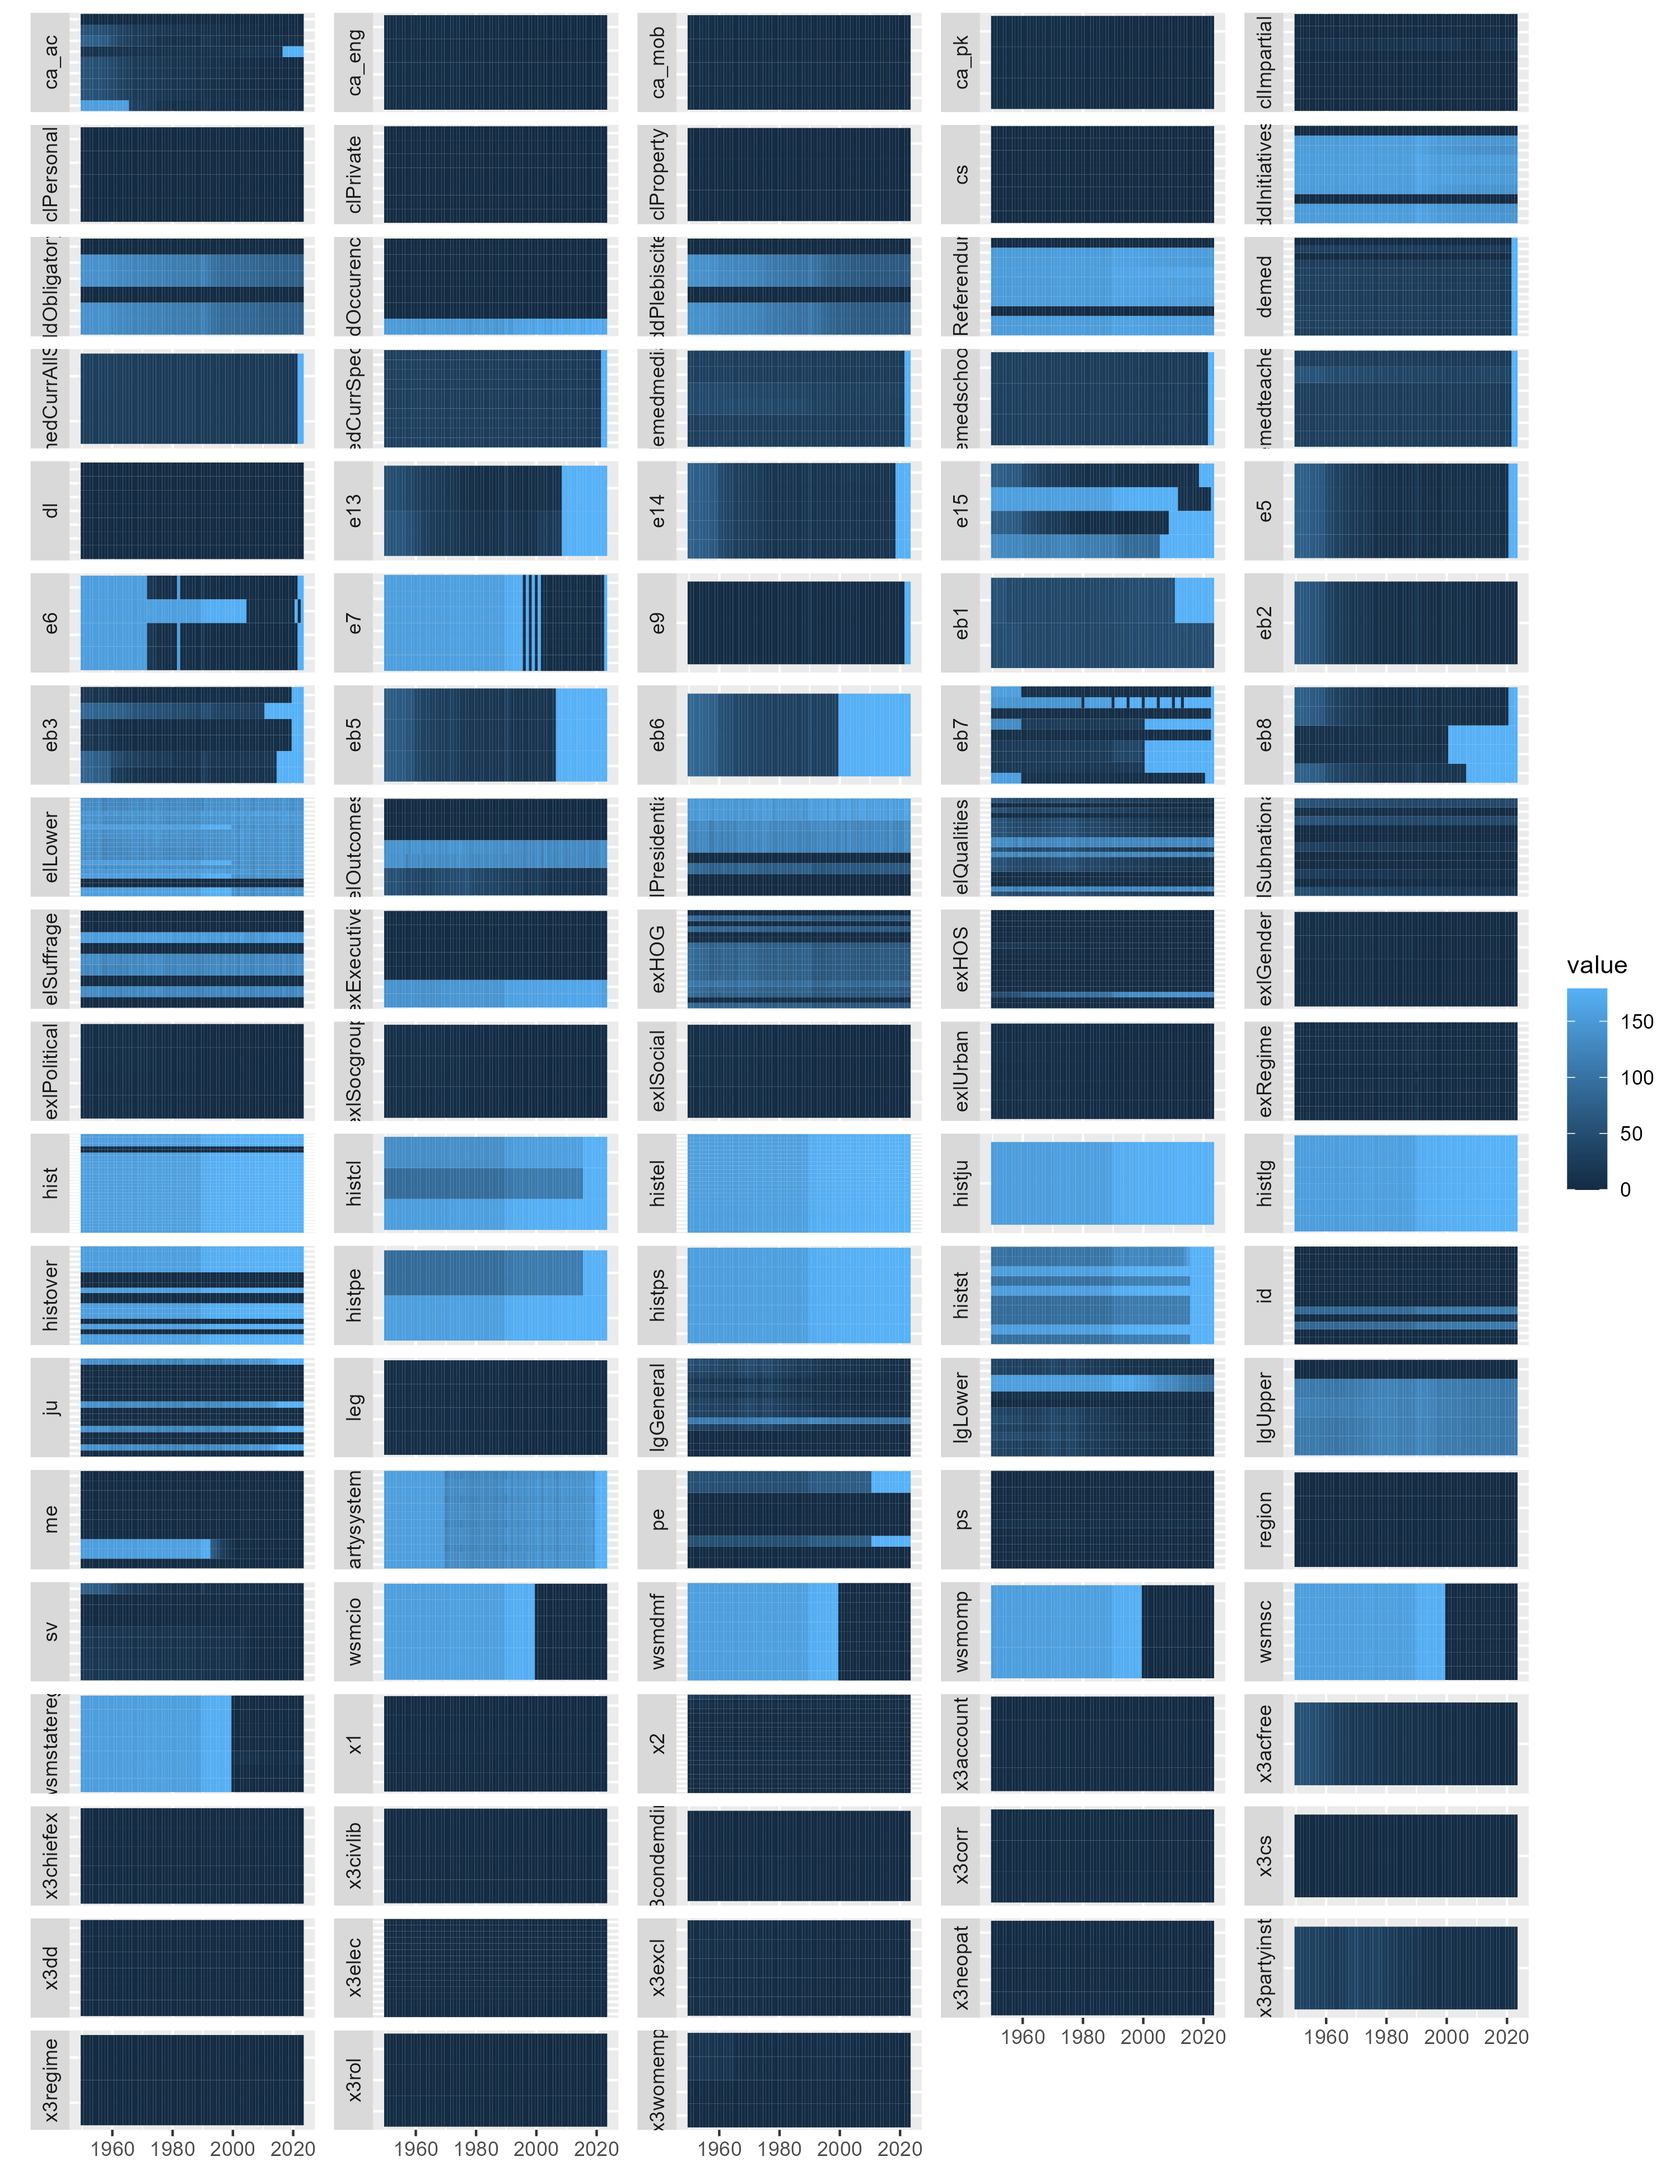
\includegraphics[width=1\textwidth]{1_nas.png}
  \caption{Conteo de nulos por año y agrupador de variables}
\end{figure}

\subsection{Análisis de variable objetivo}

\begin{figure}[H]
  \centering  
  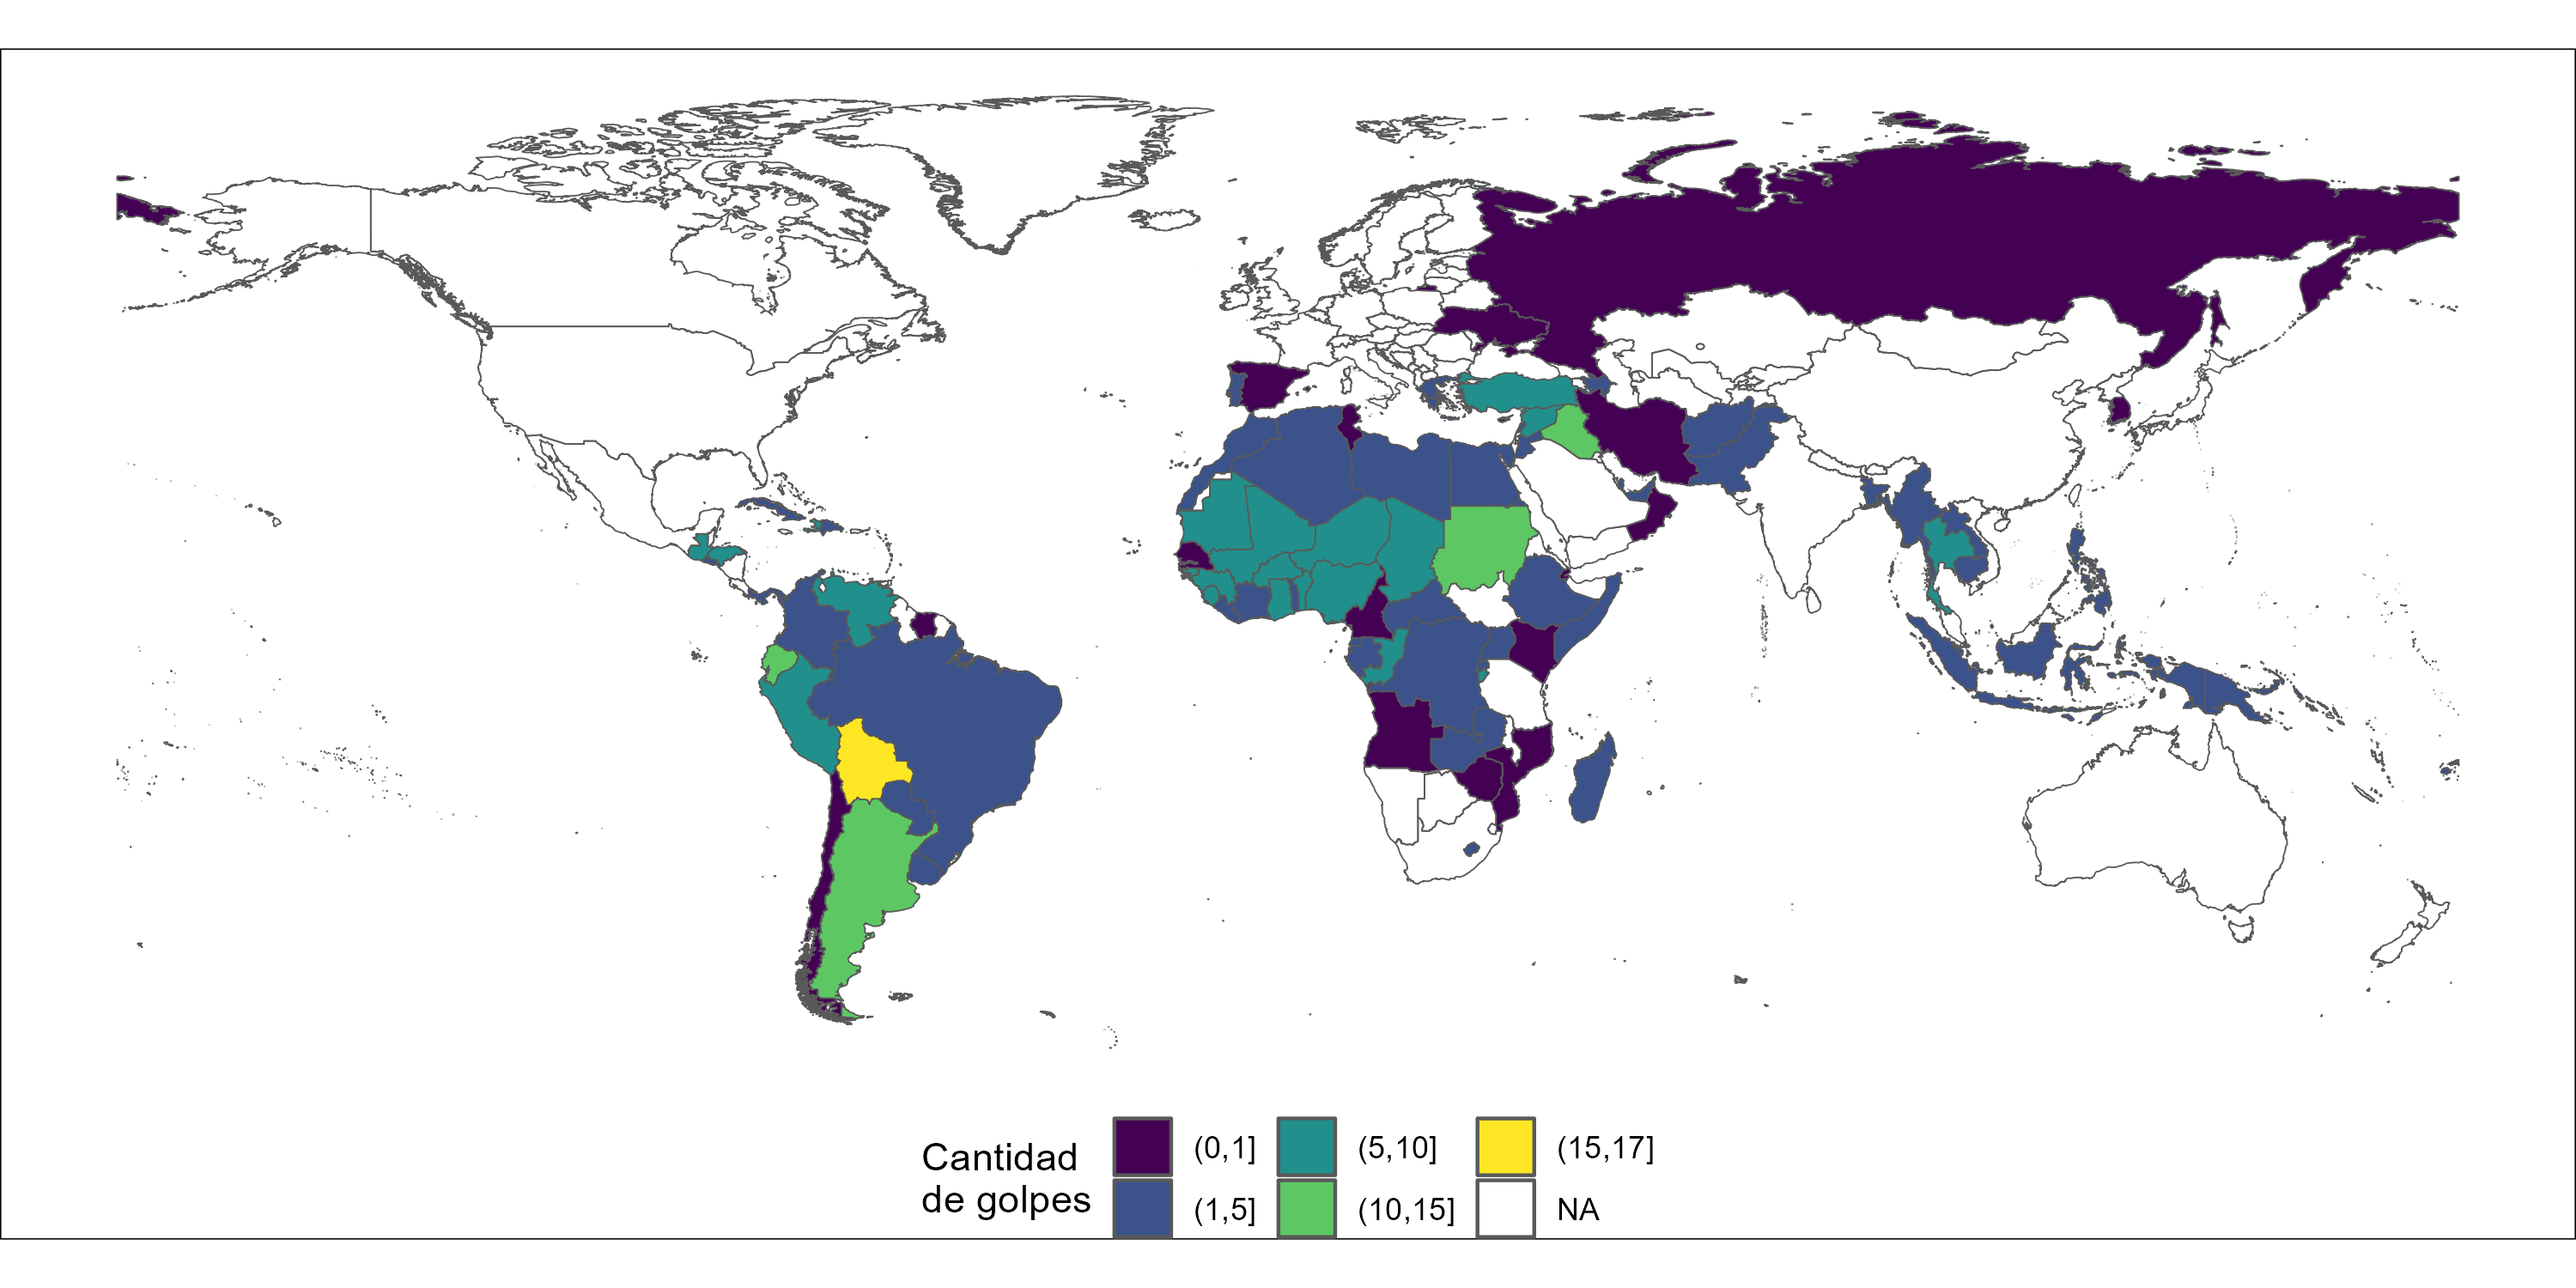
\includegraphics[width=1\textwidth]{2_golpes.png}
  \caption{Conteo de golpes de estado en el mundo}
\end{figure}


\section{Preprocesamiento de los datos}

\textit{Cargar el dataset con los datos para cada sujeto y los nombres y coordenadas 
de las regiones cerebrales a las que se les registró la actividad. Reportar cuántos sujetos y cuántos estados de sueño se observan en el conjunto de
datos.}

\printbibliography

\end{document}